\section{The Parser}

\subsection{Modified EBNF}

\setlength{\grammarparsep}{8pt plus 1pt minus 1pt} % increase separation between rules
\setlength{\grammarindent}{10em} % increase separation between LHS/RHS

Some modifications were applied to the original EBNF. Some of
the modifications were either motivated by improved user
experience, a more uniform mechanism and others to reduce
complexity further down the pipeline.

\begin{center}
\begin{grammar}
<Letter> ::= `A'-`Z' | `a'-`z'

<Digit> ::= `0'-`9'

<Hex> ::= `A'-`F' | `a'-`F' | <Digit>

<Identifier> ::= <Letter> \{`\_' | <Letter> | <Digit>\}

<BooleanLiteral> ::= `true' | `false'

<IntegerLiteral> ::= <Digit> \{<Digit>\}

<FloatLiteral> ::= <Digit> \{<Digit>\} `.' <Digit> \{<Digit>\}

<ColorLiteral> ::= `\#' <Hex> <Hex> <Hex> <Hex> <Hex> <Hex>

<ArrayLiteral> ::= `[' [<Epxr> \{`,' <Epxr>\}] `]'

<PadWidth> ::= `\_\_width'

<PadHeight> ::= `\_\_height'

<PadRead> ::= `\_\_read' <Epxr> `,' <Epxr>

<PadRandomInt> ::= `\_\_random\_int' <Epxr>

<Literal> ::= <BooleanLiteral>
\alt <IntegerLiteral>
\alt <FloatLiteral>
\alt <ColorLiteral>
\alt <ArrayLiteral>
\alt <PadWidth>
\alt <PadHeight>
\alt <PadRead>
\alt <PadRandomInt>

<Type> ::= (`bool' | `int' | `float' | `color') [ `[' <IntegerLiteral> `]' ]

<SubEpxr> ::= `(' <Epxr> `)'

<Variable> ::= <Identifier>

<ArrayAccess> ::= <Identifier> `[' <Epxr> `]'

<FunctionCall> ::= <Identifier> `(' [<Epxr> \{`,' <Epxr>\}] `)'

<Epxr> ::= <LogicOr> [`as' <Type>]

<LogicOr> ::= <LogicAnd> \{`or' <LogicAnd>\}

<LogicAnd> ::= <Equality> \{`and' <Equality>\}

<Equality> ::= <Comparison> \{(`==' | `!=') <Comparison>\}

<Comparison> ::= <Term> \{(`<' | `<=' | `>' | `>=') <Term>\}

<Term> ::= <Factor> \{(`+' | `-') <Factor>\}

<Factor> ::= <Unary> \{(`*' | `/') <Unary>\}

<Unary> ::= (`-' | `not') <Unary> | <Primary>

<RefExpr> ::= <Variable>
\alt <ArrayAccess>
\alt <FunctionCall>

<Primary> ::= <Literal>
\alt <SubExpr>
\alt <RefExpr>

<Program> ::= \{<Stmt>\}

<Stmt> ::= <Block>
\alt <VaribaleDecl> `;'
\alt <FunctionDecl>
\alt <Assignment> `;'
\alt <PrintStmt> `;'
\alt <DelayStmt> `;'
\alt <WriteBoxStmt> `;'
\alt <WriteStmt> `;'
\alt <ClearStmt> `;'
\alt <IfStmt>
\alt <ForStmt>
\alt <WhileStmt>
\alt <ReturnStmt> `;'

<Block> ::= `\{' \{<Stmt>\} `\}'

<VariableDecl> ::= `let' <Identifier> `:' <Type> `='
<Epxr>

<FormalParam> ::= <Identifier> `:' <Type>

<FunctionDecl> ::= `fun' <Identifier> `(' [ <ForamlParam>
\{`,' <FormalParam>\}] `)' `->' <Type> <Block>

<Assignment> ::= <Identifier> [`[' <Epxr> `]'] `='
<Epxr>

<PrintStmt> ::= `\_\_print' <Epxr>

<DelayStmt> ::= `\_\_delay' <Epxr>

<WriteBoxStmt> ::= `\_\_write\_box' <Epxr>`,'
<Epxr>`,'<Epxr>`,' <Epxr>`,'<Epxr>

<WriteStmt> ::= `\_\_write' <Epxr>`,' <Epxr>`,'<Epxr>

<ClearStmt> ::= `\_\_clear' <Epxr>

<IfStmt> ::= `if' `(' <Expr> `)' <Block> [`else' <Block>]

<ForStmt> ::= `for' `(' [<VariableDecl>] `;' <Expr> `;'
[<Assignment>] `)' <Block>

<WhileStmt> ::= `while' `(' <Expr> `)' <Block>

<ReturnStmt> ::= `return' <Expr>
\end{grammar}
\end{center}

\subsubsection{Improved Precedence}\label{sss:improvedprec}

So, the minor changes which improve programmer usability are the
additions of a number of other expression stages, such as
$\langle$LogicOr$\rangle$, $\langle$LogicAnd$\rangle$, etc. The
main reason for the addition of such rules is to further enforce
a more natural operation precedence. For example a programmer
often expects that comparison operators such as \texttt{<} and
\texttt{>} bind tighter than \texttt{and} or \texttt{or}, hence
the compiler needs to make sure that comparison operators are
executed before logical operators, and this can be enforced by
the grammar itself hence the changes.

\subsubsection{Better Arrays}\label{sss:secarrays}

The way arrays were being implemented in the original grammar
was very restrictive. Instead an approach for treating arrays as
their own type and literal was taken up.

The $\langle$Type$\rangle$ and $\langle$Literal$\rangle$
productions were augmented to improve array support. This helped
simplify the $\langle$Identifier$\rangle$ (in the original EBNF)
, $\langle$VariableDecl$\rangle$ and
$\langle$FormalParam$\rangle$ productions. Additionally, this
opens up further support for more complicated types later on.

For example, the $\langle$Type$\rangle$ can be further augmented
to support more types.

\begin{grammar}

<StructField> ::= <Identifier> `:' <Type>

<Struct> ::= `struct' <Identifier> `\{' \{<StructField> `;'\} `\}'

<TypeDecl> ::= <Struct>

<Base> ::= (`bool' | `int' | `float' | `color')

<Array> ::= <Type> `[' <IntegerLiteral> `]'

<Pointer> ::= <Type> `*'

<Type> ::= <Identifier>
\alt <Base>
\alt <Array>
\alt <Pointer>
\end{grammar}

Note that we are indeed repeating $\langle$ForamlParam$\rangle$
but this is not really a problem. When it comes to specification
repetition which improves clarity is ``good'' repetition.

\label{sss:primitive}Additionally, some of the ground work for
these improvements has already been laid out in the internal
type system see \listref{internaltypesys} and
\listref{primitive}.

\lstinputlisting[
linerange={185-197}, caption={Mechanism for internally storing
    types within the compiler
(parl/Core.hpp)}, label=lst:internaltypesys
]{parl/Core.hpp}

\begin{lstlisting}[caption={The Primitive structure
(parl/Core.hpp)}, label=lst:primitive]
struct Primitive {
    template <typename T>
    [[nodiscard]] bool is() const {
        return std::holds_alternative<T>(data);
    }

    template <typename T>
    [[nodiscard]] const T &as() const {
        return std::get<T>(data);
    }

    ...

    bool operator!=(Primitive const &other) {
        return !operator==(other);
    }

    std::variant<std::monostate, Base, Array> data{};
};
\end{lstlisting}

The \texttt{box} type is a special type of pointer
object which has value semantics that is it behaves
as though it were the object it contains.

This is critical because self-referential types like the
$\langle$Array$\rangle$ as described above are not easily
representable within \CC{} since, something like
\listref{unboundedsize}, is not allowed.

\begin{lstlisting}[caption={An size unbounded type in \CC{}
(parl/Core.hpp)}, label=lst:unboundedsize]
struct SelfRef;

struct Container {
    Other other;
    SelfRef ref;
};

struct Primitive {
    std::variant<std::monostate, Container> data{};
};
\end{lstlisting}

This is because the \CC{} compiler is incapable of determining
the size of said type at compile-time. Hence, a pointer for said
type is required. And the pointer wrapper \texttt{box<>} allows
it to be copied as tough it were a value.

The \texttt{box<>} type is attributed to Jonathan Müller were he
discuss the exact issue described above on his
\href{https://www.foonathan.net/2022/05/recursive-variant-box/}{
blog}, \texttt{foonathan}.

These changes to type also require additional, changes to how
variables are referenced in expressions hence why
$\langle$RefExpr$\rangle$ was added. It also ensure that in the
future more complicated referencing such as
\texttt{object.something} (\texttt{struct} member referencing)
is possible.

Finally, the $\langle$ArrayLiteral$\rangle$ has been improved to
support expressions instead of just only literals.

\subsubsection{Removing Eye-Candy}\label{eyecandy}

Adding this system however, significantly increases the
complexity of semantic analysis.

Because of this the slight syntax sugar of being able to have
the following two conveniences \texttt{let a: int[] = [1,1,1];}
and \texttt{let a: int[3] = [1];} has been dropped.

This is because such syntax not only complicates the grammar but
it also significantly increases the complexity of semantic
analysis.

The best way to handle this is to have a de-sugaring \& type
inference sub-phase before type checking, within the semantic
analysis phase.

\subsection{Parsing \& The Abstract Syntax Tree}

The AST is the data structure which is produced by the parser.
The nodes of the AST are in fact almost a one-to-one
representation of the productions in the grammar, for example
see \listref{funccallast}.

\lstinputlisting[
linerange={140-148}, caption={The \texttt{FunctionCall} AST node class
(parl/AST.hpp)}, label=lst:funccallast
]{parl/AST.hpp}

The only significant difference in these nodes in the
\texttt{Position} field. This get populated by the parser using
the location of a token in the original source file. This is
again critical for adequate error messaging later in the
semantic analysis phase.

\lstinputlisting[
linerange={158-167}, caption={The \texttt{Binary} AST node class
(parl/AST.hpp)}, label=lst:binaryast
]{parl/AST.hpp}

\lstinputlisting[
linerange={169-177}, caption={The \texttt{Unary} AST node class
(parl/AST.hpp)}, label=lst:unaryast
]{parl/AST.hpp}

Apart from these the only other real difference is the use of a
\texttt{Binary} and \texttt{Unary} node see \listref{binaryast}
and \listref{unaryast}, instead of a node for each type of the
grammar rules discussed above in \ref{sss:improvedprec}. This is
because the reason for said rules was precedence and precedence
within the AST is actually described by the structure of the
tree itself not the node types.

Additionally, a number of the nodes override the
\texttt{accept()} method specified by the pure virtual class
\texttt{Node}. This is the basis for the Visitor pattern which
apart form the parser is the backbone of the remaining phases.

\subsection{The Actual Parser}

The parser is split into four main sections.

\begin{itemize}
    \item AST Generation
    \item Token Buffering
    \item Token Matching
    \item Error Handling/Recovery
\end{itemize}

\subsubsection{Token Buffering}

The parser requires access to the tokens for proper functioning.
Additionally, sometimes the parser requires more than one token
as the case deciding on whether an identifier is just a variable
or a function call. This is quite easy to implement if the
parser has available to it at initialisation all the tokens.

However, as described in \ref{sss:runnerlexer}. This is not the
case the parser requests token on demand from lexer which it has
a reference. This of course means that the machinery for
handling tokens is a bit more complicated due to requiring
lookahead.

To solve this issue a window-based approach was adopted. The
parser has a moving buffer/window called \texttt{mTokenBuffer}
and whose size is specified at compile-time using a C-style
macro \texttt{\#define LOOKAHEAD (2)}. The core methods for this
aspect of the parser are \texttt{moveWindow()} and
\texttt{nextToken()}, see \listref{tokenbuffering}.

\lstinputlisting[ linerange={1076-1095}, caption={The
\texttt{moveWindow()} and \texttt{nextToken()} Parser methods
(parser/Parser.cpp)},
label=lst:tokenbuffering]{parser/Parser.cpp}

Additionally, note that within \texttt{nextToken()} the
whitespace and comments are being explicitly ignored.

This might lead to further minor improvement. Specifically,
comments can be integrated into the AST. This basically allows
printing visitors or, formatting visitors properly format the
code whilst still preserving any comments created by
programmers.

\subsubsection{Token Matching}

The previous methods all facilitate the more important token
matching methods which are:

\begin{itemize}
    \item \texttt{peek()},
    \item \texttt{advance()},
    \item \texttt{previous()},
    \item \texttt{isAtEnd()},
    \item \texttt{peekMatch()},
    \item \texttt{match()},
    \item and, \texttt{consume()}.
\end{itemize}

Arguably, the most improtant of these methods is
\texttt{consume()}, it takes in a token type and a error message
if the specified token type is not matched, see
\listref{consume}.

\lstinputlisting[linerange={96-107}, caption={The
\texttt{consume()} Parser methods (parser/Parser.hpp)},
label=lst:consume]{parser/Parser.hpp}

The main reason for the templating of such a method is to
provide an easy interface for formattable strings using
\href{https://github.com/fmtlib/fmt}{fmtlib}. The main feature
this library provides is the ability to specify placeholders
in the string itself using \texttt{\{\}}. Usage of this
functionality is demonstrated in the AST generator methods, see
\listref{consumeusage}.

\lstinputlisting[linerange={522-527}, caption={The Usage of the
\texttt{consume()} method in the \texttt{formalParam()}
generator method (parser/Parser.cpp)},
label=lst:consumeusage]{parser/Parser.cpp}

The \texttt{peekMatch()} method is a simple method which returns
true if at least one of the provided token types match. The main
usage for this is cases where more than different token is valid
option for example such is the case for
$\langle$Comparison$\rangle$ production. \texttt{match()} is a
simple extension of \texttt{peekMatch()} which consumes the
token if it matches.

The methods \texttt{advance()}, \texttt{previous()} and
\texttt{isAtEnd()} are quite self explanatory.
\texttt{advance()} moves the buffer window one step forward,
\texttt{previous()} returns the last consumed token, and
\texttt{isAtEnd()} checks whether or not the parser has reached
an End of File token.

\texttt{peek()} is also very simple it allows the parser to see
the token without consuming it. However, since the parser might
need to lookahead peek() supports an offset. The only issue is
that all calls to \texttt{peek()} have to be checked to ensure
that valid access, see \listref{peek}. This is done using \texttt{abort\_if()}
function which prints an error message an aborts the program.
This is very similar to a \texttt{static\_assert} however, it is
has to be performed at runtime, see \listref{abortif}.

\lstinputlisting[linerange={1101-1109}, caption={The
\texttt{peek()} Parser method (parser/Parser.cpp)},
label=lst:peek]{parser/Parser.cpp}

\lstinputlisting[linerange={13-41}, caption={The abort
functionality present in the codebase (parl/Core.hpp)},
label=lst:abortif]{parl/Core.hpp}

Note that since the usage of \texttt{abort()} and
\texttt{abort\_if()} is internal to the code, it only makes
sense for these functions to be enabled during debug builds
only. Hence, the implementation are enclosed between an
\texttt{\#ifdef, \#else, \#endif} macro. When \texttt{NDEBUG}
which stand for no-debug is defined the function bodies are
hollowed out allowing the \CC{} compiler to optimise them out.

\subsubsection{Error Handling/Synchronization}

Error handling and synchronization is a critical part of the
parser. With regards to developer productivity, having
meaningful errors is extremely valuable. But apart from that
being able see all the errors in a file is also crucial. This
means that a developer will waste less time re-running the
compiler to find all the errors present in the source code. This
processes is referred to as
\href{https://craftinginterpreters.com/parsing-expressions.html#synchronizing-a-recursive-descent-parser}{Synchronization}
by the author of
\href{https://craftinginterpreters.com/}{Crafting Interpreters},
Robert Nystrom. The method for synchronization in the
\texttt{PArL} compiler was inspired by the above credited author
and his usage of Exceptions as an unrolling primitive although
unorthodox is very simple to implement and has in fact been used
in the parser and also later stages of the compiler with success.

\begin{lstlisting}[caption={The \texttt{ParseSync} exception and
the \texttt{error()} method which kickstarts the synchronization
process (parser/Parser.hpp)}, label=lst:synckickstart]
class SyncParser : public std::exception {};

...

template <typename... T>
void error(fmt::format_string<T...> fmt, T&&... args) {
    mHasError = true;

    Token violatingToken = peek();

    fmt::println(
        stderr,
        "parsing error at {}:{}:: {}",
        violatingToken.getPosition().row(),
        violatingToken.getPosition().col(),
        fmt::format(fmt, args...)
    );

    throw SyncParser{};
}
\end{lstlisting}

However, there is of course a major downside to this where
synchronization happens will affect other error messages which
are reported down stream. This of course has the possibility of
producing false positives. However, in this case error handling
is only best-effort and therefore the possibility of false
positives accepted. The basic process of synchronizing is
consuming as many tokens as possible until the parser reaches a
token which it believes to be a good restarting point, see
\listref{sync}.

\lstinputlisting[linerange={1159-1205}, caption={The
\texttt{synchronize()} method in the Parser class
(parser/Parser.cpp)}, label=lst:sync]{parser/Parser.cpp}

Finally, the most natural choice for capturing
\texttt{ParserSync} is in AST generator methods responsible for
generating statement nodes, those being \texttt{program()} and
\texttt{block()}.

\subsubsection{AST Generator Methods}

Finally, the bulk of the parser is actually the generator
methods which actually build the AST. These methods are not that
complicated and they follow the specified grammar faithfully.

See, \listref{ifstmt} for an example of such a method and see
\listref{methodslist} for a full list of the methods.

\lstinputlisting[linerange={385-419}, caption={The
\texttt{ifStmt()} node generator method in the Parser class
(parser/Parser.cpp)}, label=lst:ifstmt]{parser/Parser.cpp}

\begin{lstlisting}[caption={The main body of methods in the
Parser class (parser/Parser.hpp)}, label=lst:methodslist]
std::unique_ptr<core::Type> type();

std::unique_ptr<core::Program> program();
std::unique_ptr<core::Stmt> statement();
std::unique_ptr<core::Block> block();
std::unique_ptr<core::VariableDecl> variableDecl();
std::unique_ptr<core::Assignment> assignment();
std::unique_ptr<core::PrintStmt> printStatement();
std::unique_ptr<core::DelayStmt> delayStatement();
std::unique_ptr<core::WriteBoxStmt> writeBoxStatement();
std::unique_ptr<core::WriteStmt> writeStatement();
std::unique_ptr<core::ClearStmt> clearStatement();
std::unique_ptr<core::IfStmt> ifStmt();
std::unique_ptr<core::ForStmt> forStmt();
std::unique_ptr<core::WhileStmt> whileStmt();
std::unique_ptr<core::ReturnStmt> returnStmt();
std::unique_ptr<core::FunctionDecl> functionDecl();
std::unique_ptr<core::FormalParam> formalParam();

std::unique_ptr<core::PadWidth> padWidth();
std::unique_ptr<core::PadHeight> padHeight();
std::unique_ptr<core::PadRead> padRead();
std::unique_ptr<core::PadRandomInt> padRandomInt();
std::unique_ptr<core::BooleanLiteral> booleanLiteral();
std::unique_ptr<core::ColorLiteral> colorLiteral();
std::unique_ptr<core::FloatLiteral> floatLiteral();
std::unique_ptr<core::IntegerLiteral> integerLiteral();
std::unique_ptr<core::ArrayLiteral> arrayLiteral();
std::unique_ptr<core::SubExpr> subExpr();
std::unique_ptr<core::Variable> variable();
std::unique_ptr<core::ArrayAccess> arrayAccess();
std::unique_ptr<core::FunctionCall> functionCall();

std::unique_ptr<core::Expr> expr();
std::unique_ptr<core::Expr> logicOr();
std::unique_ptr<core::Expr> logicAnd();
std::unique_ptr<core::Expr> equality();
std::unique_ptr<core::Expr> comparison();
std::unique_ptr<core::Expr> term();
std::unique_ptr<core::Expr> factor();
std::unique_ptr<core::Expr> unary();
std::unique_ptr<core::Expr> primary();
\end{lstlisting}

\subsection{Pretty? Printing}

\subsubsection{Using Parser in the Runner}

The parser is used in the runner and assuming that the parser
does not encounter any errors and the \texttt{mParserDbg} flag
is set it can be used to print the AST using a
\texttt{PrinterVisitor}.

\lstinputlisting[linerange={117-127}, caption={The parse segment
of the \texttt{run()} method in the Runner class
(runner/Runner.cpp)}]{runner/Runner.cpp}

Calling the produced \texttt{PArL} binary with the \texttt{-p}
flag will set the \texttt{mParserDbg}, see \figref{test9} and
\figref{parseeg}.

\begin{figure}[H]
\centering
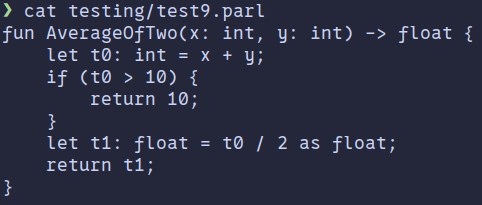
\includegraphics[width=\linewidth]{test9.png}
\caption{\texttt{cat} of the test9.parl}
\label{fig:test9}
\end{figure}

\begin{figure}[H]
\centering
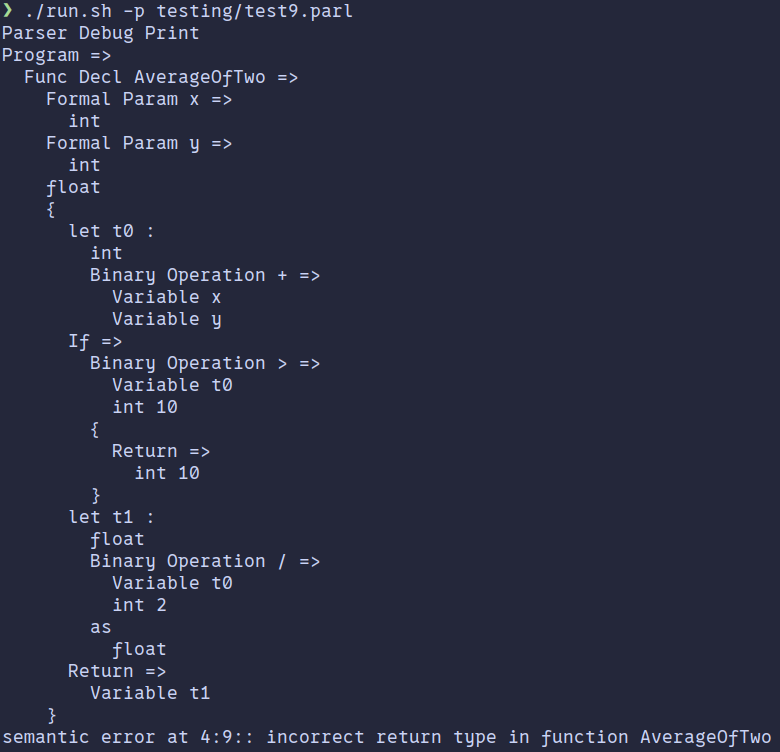
\includegraphics[width=\linewidth]{printervisitoreg.png}
\caption{The AST generated by the syntactically correct program
in test9.parl}
\label{fig:parseeg}
\end{figure}

\lstinputlisting[linerange={104-110}, caption={The
\texttt{debugParsing()} method in the Runner class
(runner/Runner.cpp)},label=lst:debugparsing]{runner/Runner.cpp}

The \texttt{PrinterVisitor} used in \listref{debugparsing} is
a specialization of the pure virtual \texttt{Visitor} class
in parl/Visitor.hpp.

\begin{lstlisting}[caption={A segment of the pure virtual
\texttt{Visitor} class (parl/Visitor.hpp)},
label=lst:genericvisitor]
...

struct ClearStmt;
struct Block;
struct FormalParam;
struct FunctionDecl;
struct IfStmt;
struct ForStmt;
struct WhileStmt;
struct ReturnStmt;
struct Program;

class Visitor {
   public:
    virtual void visit(Type*) = 0;
    virtual void visit(Expr*) = 0;
    virtual void visit(PadWidth*) = 0;
    virtual void visit(PadHeight*) = 0;
    virtual void visit(PadRead*) = 0;
    virtual void visit(PadRandomInt*) = 0;
    virtual void visit(BooleanLiteral*) = 0;
    virtual void visit(IntegerLiteral*) = 0;
    virtual void visit(FloatLiteral*) = 0;

...
\end{lstlisting}

Due to the way \CC{} handles symbols, the classes which the
visitor can visit must be forward declared manually, see
\listref{genericvisitor}. If no such forward declaration is
made, the compiler will complain about the \texttt{Visitor} and
the \texttt{AST} classes being cyclically dependent.

Additionally, any inheriting visitor such as the
\texttt{PrinterVisitor} can hold state. In fact, this is where
the true power of visitors arises. Being able to hold state
means that complex computations can be carried out on the AST.
For example the \texttt{PrinterVisitor} although simple makes
use of a single variable \texttt{mTabCount}, see
\listref{printnode}, which it uses to affect how much
indentation should be used in printing, allowing us to visualise
the AST.

\lstinputlisting[linerange={45-53}, caption={The
\texttt{visit(core::PadRead*)} method in the
\texttt{PrinterVisitor}
(parser/PrinterVisitor.cpp)},label=lst:printnode]{parser/PrinterVisitor.cpp}
